% /!\ Ctrl+H "\item ~[" / "\\ ["=> "\item ~[" / "\\ ~["
% TODO!? put in italic the "didascalies" in []
% TODO? give policies options here instead of referring to "this spreadsheet"
Below, we provide the generic questionnaire (based on the U.S. version), which roughly corresponds to the \textit{Eu} questionnaire as well as the combination of the \textit{US1} and \textit{US2} questionnaire. The main difference between Europe and the U.S. is that we split the \textit{US2} sample into four random branches to include some treatments before the Section \ref{subsec:questionnaire_GCS} on the GCS. Besides the control group, the treatments are: information regarding the support of Americans for the GCS and NR, an open-ended field, and a closed question on the pros and cons of the GCS. The pros and cons of the GCS are also asked in Eu (likewise, either as an open-ended field or a question), but only in Section \ref{subsec:questionnaire_perceptions}, after the support. 

At each section or question, we specify in square brackets in which questionnaires it is present (\textit{US1}, \textit{US2} and/or \textit{Eu}) as well as country specificities. Figures \ref{fig:flow_Eu}-\ref{fig:flow_US2} also allow understanding the structure of each questionnaire. Qualtrics and Word versions of the questionnaires in each language are available on our \href{https://github.com/bixiou/global_tax_attitudes/tree/main/questionnaire}{public repository}, together with a spreadsheet that summarizes country specificities and our sources.

\begin{figure}[h!]
    \caption{\textit{Eu} survey structure}\label{fig:flow_Eu}
    \makebox[\textwidth][c]{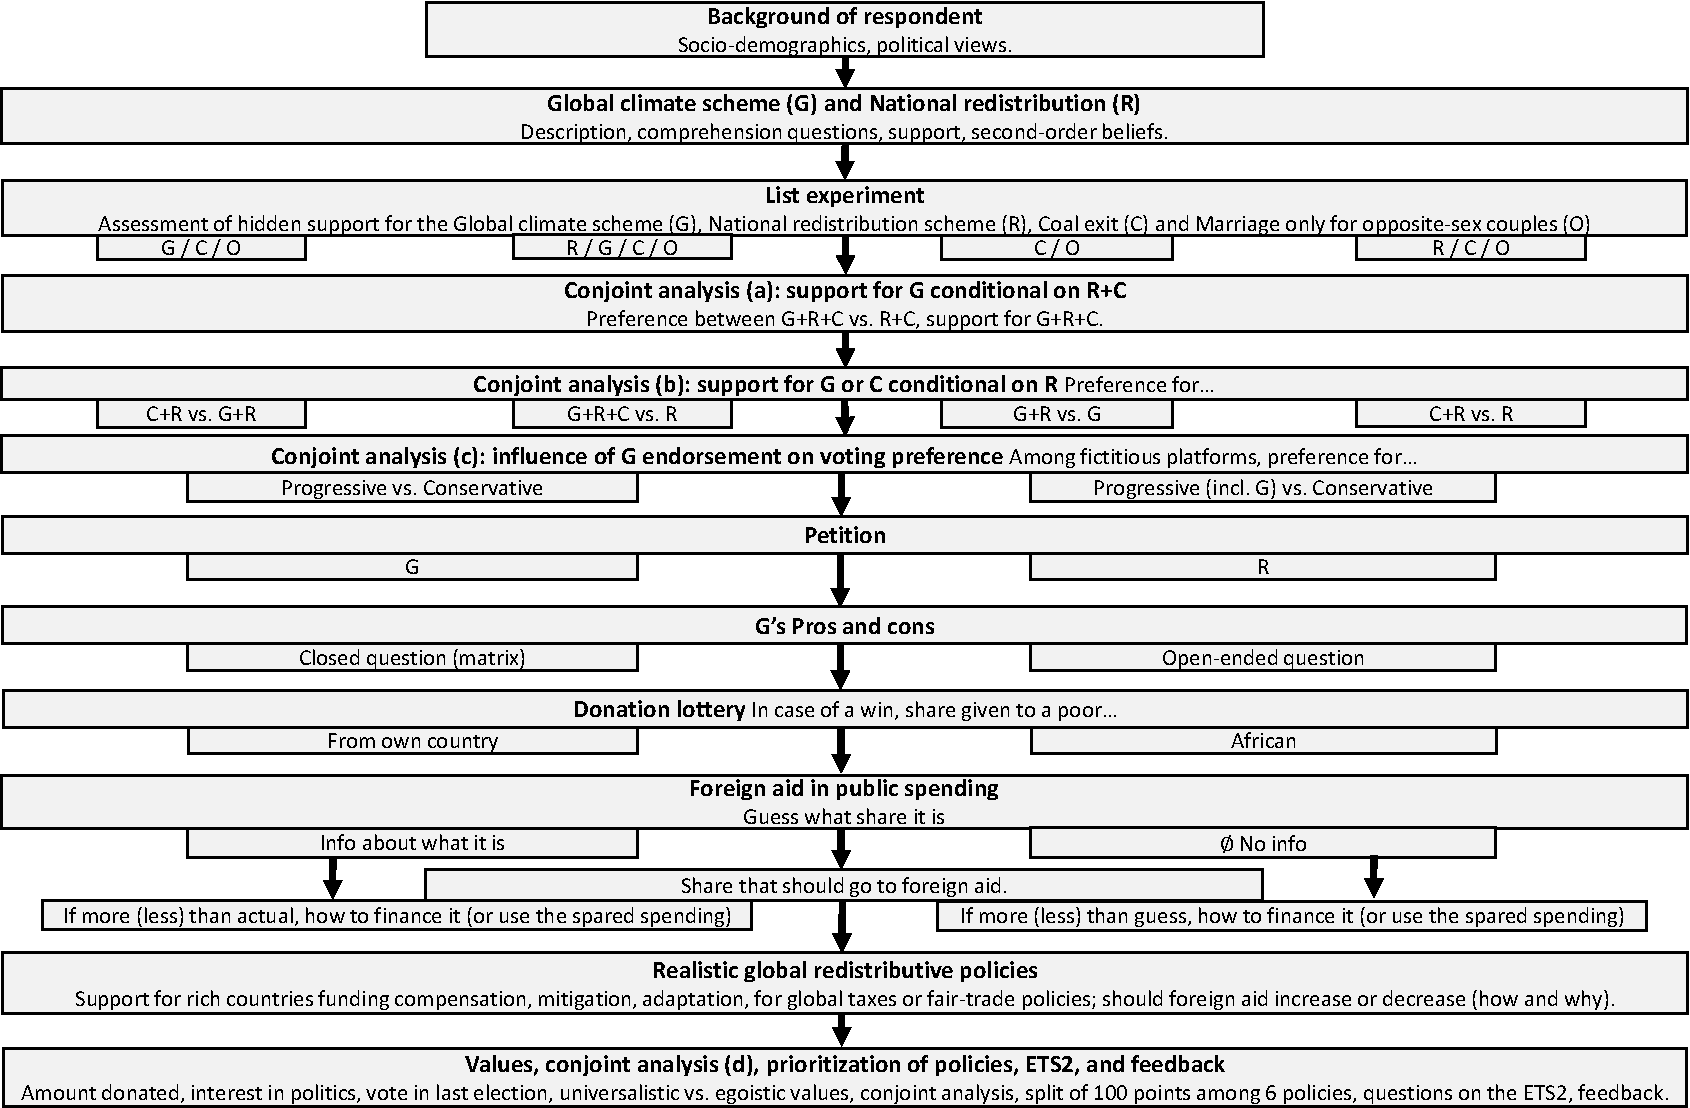
\includegraphics[width=\textwidth]{../questionnaire/survey_flow_EU.pdf}} 
\end{figure}

\begin{figure}[h!]
    \caption{\textit{US1} survey structure}\label{fig:flow_US1}
    \makebox[\textwidth][c]{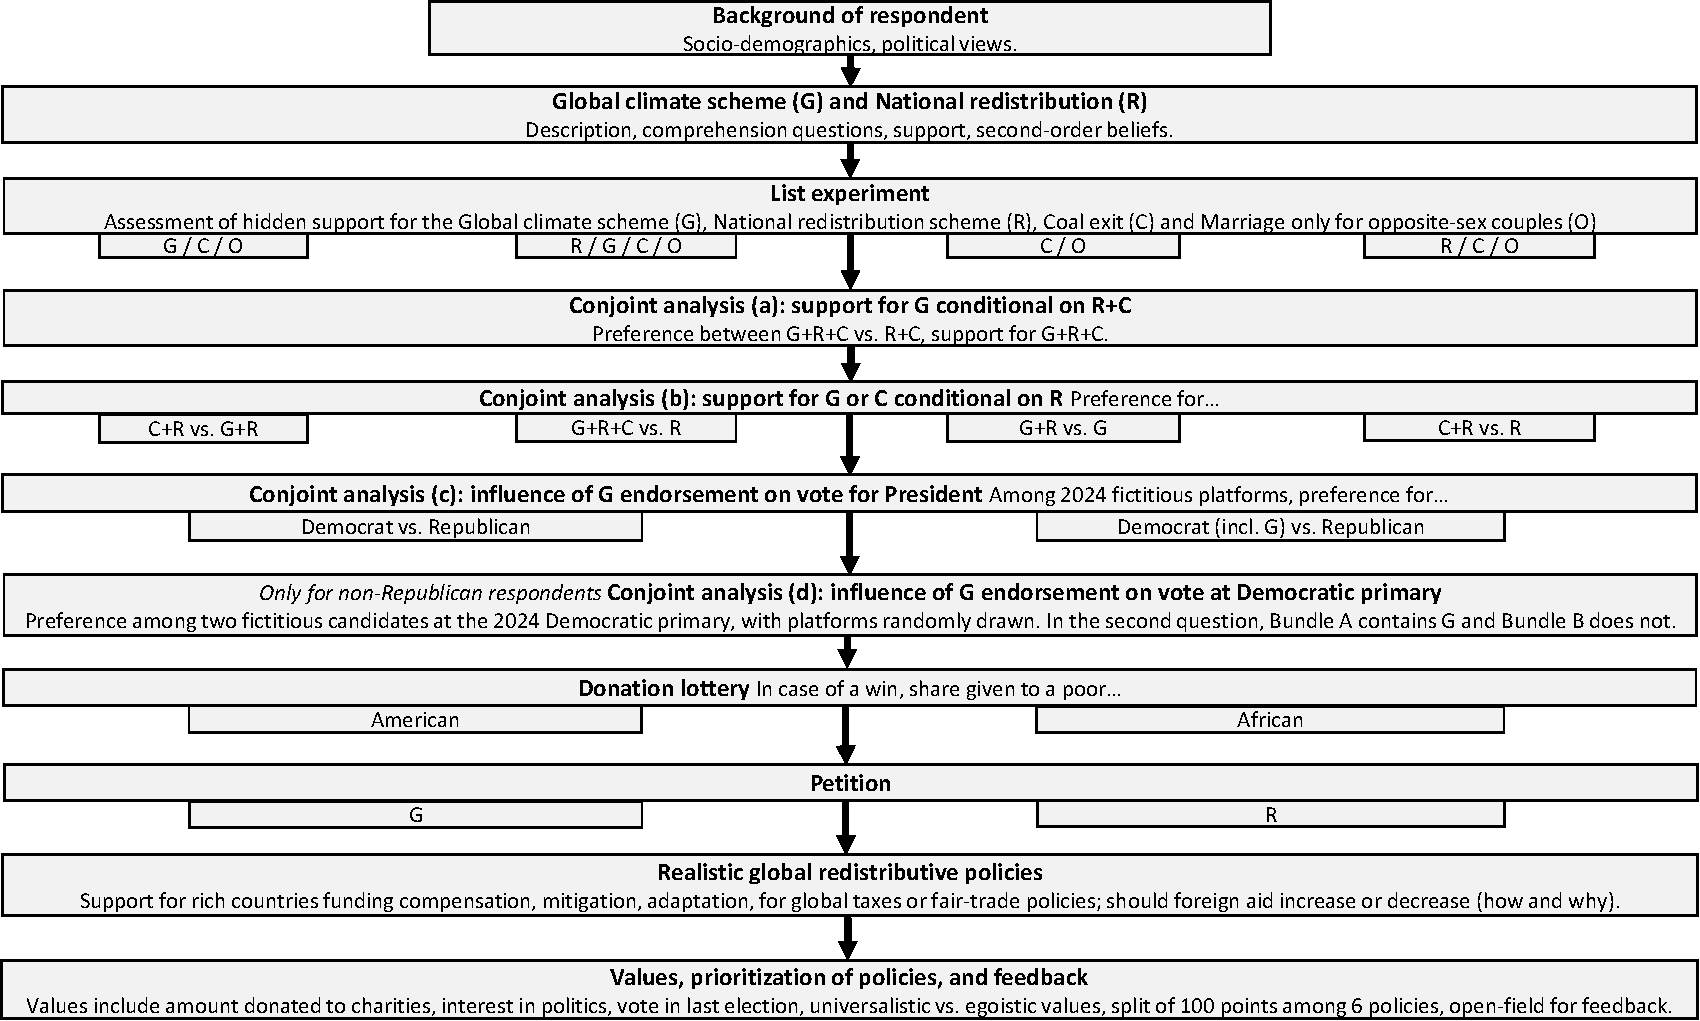
\includegraphics[width=\textwidth]{../questionnaire/survey_flow_US1.pdf}} 
\end{figure}

\begin{figure}[h!]
    \caption{\textit{US2} survey structure}\label{fig:flow_US2}
    \makebox[\textwidth][c]{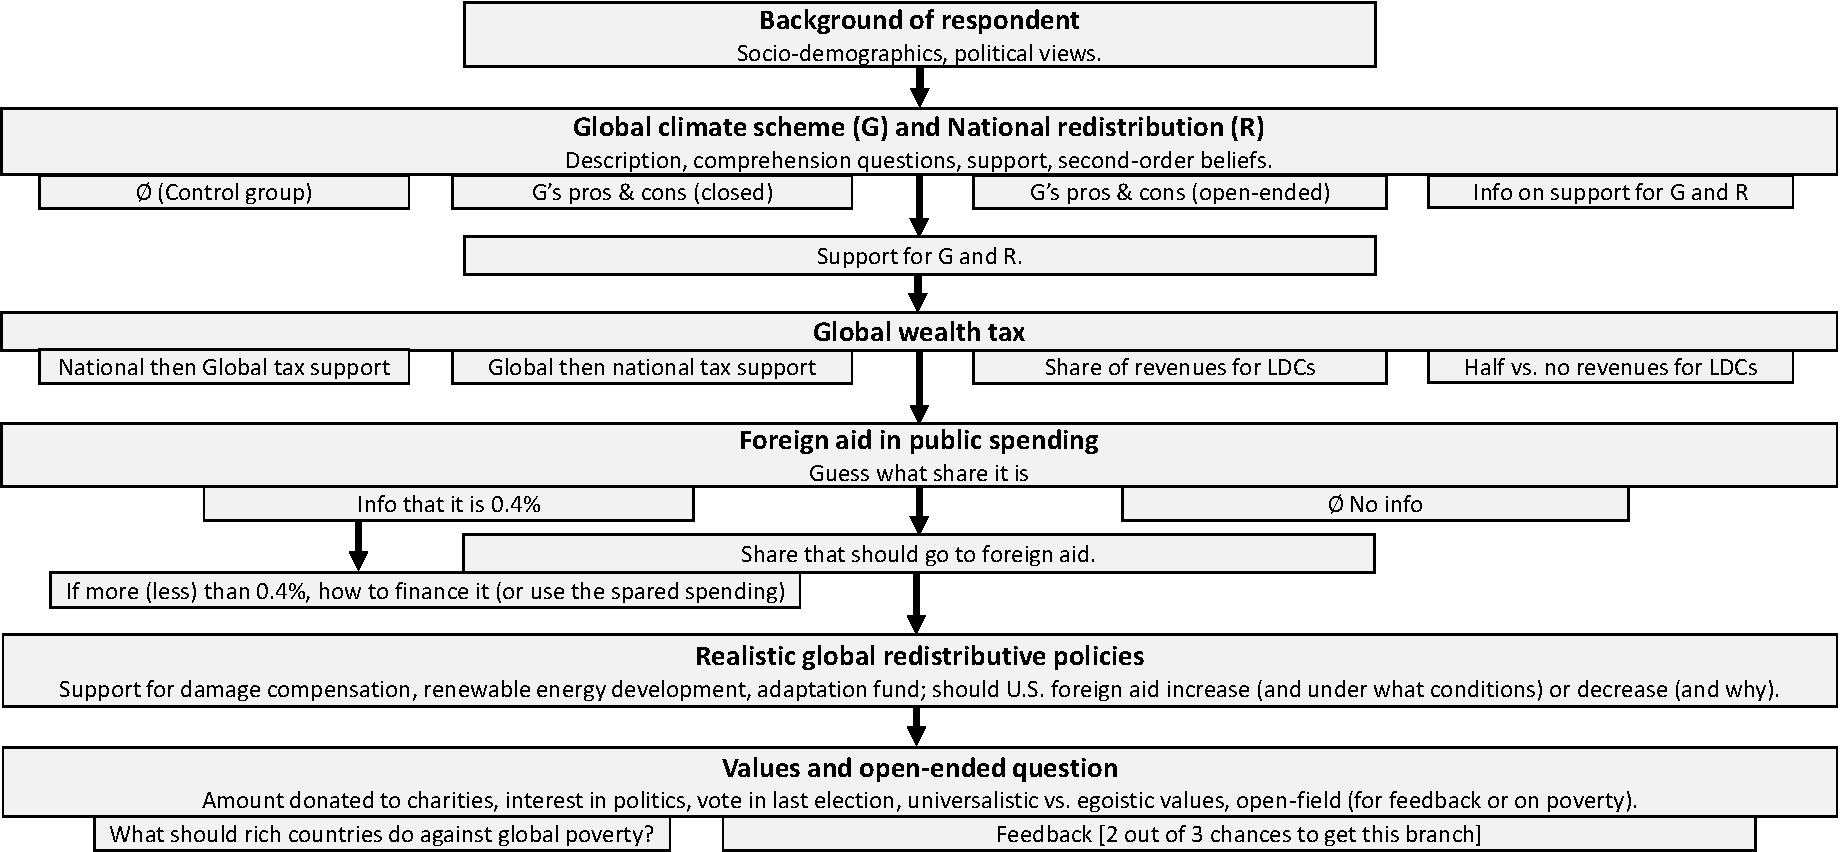
\includegraphics[width=\textwidth]{../questionnaire/survey_flow_US2.pdf}} 
\end{figure}

\clearpage
\subsection*{[\textit{Eu}, \textit{US1}, \textit{US2}] Socio-demographic characteristics}
\begin{enumerate}
\item Welcome to this survey!\\
\\
This survey is \textbf{anonymous} and is conducted \textbf{for research} purposes on a representative sample of [1,000 British people].\\
 \\
It takes [\textit{US1}, \textit{US2}: 10 to 15 min; \textit{Eu}: around \textbf{20 min}] to complete.  \\
 \\
The survey contains lotteries and awards for those who get the correct answer to some understanding questions.\\
If you are attentive and lucky, \textbf{you can win up to }[\textit{US1}, \textit{Eu}: \textbf{\$350}; \textit{US2}: \textbf{\$150}] in points. (\href{https://uvafeb.eu.qualtrics.com/WRQualtricsControlPanel/File.php?F=F_cBZAXTgNktGZbee&download=1}{See terms and conditions}).    \\
Please answer every question carefully.  \\
 \\
\textbf{Do you agree to participate in the survey?}
\\ \textit{Yes; No}
\item What is your gender?
\\ \textit{Woman; Man; Other}
\item How old are you?
\\ \textit{Below 18; 18 to 20; 21 to 24; 25 to 29; 30 to 34; 35 to 39; 40 to 44; 45 to 49; 50 to 54; 55 to 59; 60 to 64; 65 to 69; 70 to 74; 75 to 79; 80 to 84; 85 to 89; 90 to 99; 100 or above}
\item ~[\textit{Eu}] In which country do you live?
\\ \textit{France; Germany; Spain; United Kingdom; Other}
\item What is your ZIP code? [UK: What is your Outcode (the left part of your postcode, e.g. if your postcode is N7 8H7, just enter N7)?]
\item \label{q:partner} Do you live with your partner (if you have one)?
\\ \textit{Yes; No}
\item How many people are in your household? The household includes: you, the members of your family who live with you, and your dependants. %This excludes flatmates.
\\ \textit{1; 2; 3; 4; 5 or more}
\item \label{q:children} [\textit{Eu}] How many children below 14 live with you?
\\ \textit{1; 2; 3; 4 or more}
\item ~[\textit{US1}, \textit{US2}] What race or ethnicity do you identify with? (Multiple answers are possible) 
\\ \textit{White; Black or African American; Hispanic; Asian; American Indian or Alaskan Native; Natice Hawaiian or Pacific Islander; Other: \{open field\}; Prefer not to say}
\item What is the [\textit{US1}, \textit{US2}: \textit{annual}; \textit{Eu}: \textit{monthly}] gross income of your household (before withholding tax)? This includes all income: wages, self-employment earnings, Social Security benefits, pensions, investment income, welfare payments, and income from other sources. % ~[quartiles thresholds are given for the U.S. ] 
\\ ~[\textit{US1}, \textit{US2}: Items based on household total income deciles and quartiles, namely: \textit{Less than \$20,000; between \$20,001 and \$35,000; between \$35,001 and \$42,000; between \$42,001 and \$50,000; between \$50,001 and \$65,000; between \$65,001 and \$82,000; between \$82,001 and \$103,000; between \$103,001 and \$130,000; between \$130,001 and \$145,000; between \$145,001 and \$165,000; between \$165,001 and \$250,000; More than \$250,000; I prefer not to answer}; \\ \textit{Eu}: custom thresholds, taking into account household composition Questions \ref{q:partner}-\ref{q:children}, and corresponding to the country's deciles and quartiles of standard of living, cf. the sheet ``Income'' in \href{https://github.com/bixiou/global_tax_attitudes/raw/main/questionnaire/specificities.xlsx}{this spreadsheet}]
\item What is the highest level of education you have completed? 
\\ ~[\textit{Below upper secondary}, \textit{Upper secondary}, and \textit{Post secondary} are coded as the first two, middle three, and last three items, respectively. \\ \textit{US1}, \textit{US2}: \textit{Primary school or less; Eigth grade; Some high school; Regular high school diploma/GED or alternative credential; Some college, no degree; 2-year college degree or associates degree (for example: AA, AS); Bachelor's degree (for example: BA, BS); Master’s degree or above (MA, MS, MEng, MEd, MSW, MBA, MD, DDS, DVM, LLB, JD, PhD); } \\FR: \textit{École primaire / Aucun; Brevet; CAP ou BEP; Baccalauréat professionnel ou technologique; Baccalauréat général; Bac +2 (BTS, DUT, DEUG…); Bac +3 (licence…); Bac +5 ou plus (master, école d'ingénieur ou de commerce, doctorat, médecine, maîtrise, DEA, DESS...)} \\DE: \textit{Keine abgeschlossene Schulbildung / Grundschule; Untere Sekundarstufe (z.B. Haupt- oder Realschulabschluss); Erstausbildung; Beruflicher Abschluss / Ausbildung; Abitur; Zweitausbildung; Bachelor oder Fachhochschulabschluss; Master-Abschluss oder höher} \\ ES: \textit{Educación primaria / No he completado la enseñanza básica; Educación secundaria obligatoria (ESO); Formación profesional básica (FP); Formación profesional de grado medio; Bachillerato; Formación profesional de grado superior; Grado universitario; Máster/doctorado}\\ UK: \textit{Primary education or less; Some secondary school; GSCE; Vocational Upper secondary (Level 3 award, level 3 certificate, level 3 diploma, advanced apprenticeship, etc.); High school degree (A level); Higher vocational education (Level 4+ award, level 4+ certificate, level 4+ diploma, higher apprenticeship, etc.); Bachelor's Degree (BA, BSc, BEng, etc.); Postgraduate diploma or certificate, Master's Degree (MSc, MA, MBA, etc.) or Ph.D.}]
\item What is your employment status? \label{item:employment}
\\ \textit{Full-time employed; Part-time employed; Self-employed; Student; Retired; Unemployed (searching for a job); Inactive (not searching for a job)}
\item Are you a homeowner or a tenant? (Multiple answers are possible) 
\\ \textit{Tenant; Owner; Landlord renting out property; Hosted free of charge}
\item ~[If lives with partner: What is the estimated value of your household's assets (in U.S. dollars)?  \\
 If does not live with partner: What is the estimated value of your assets (in U.S. dollars)?]
   \\
Include here all your possessions (home, car, savings, etc.) net of debt. For example, if you own a house worth [\$]300,000 and you have [\$]100,000 left to repay on your mortgage, your assets are [\$]200,000.  \\
  \\
I estimate my [If lives with partner: household's] assets net of debt to be:  \\% ~[Quintiles thresholds are given for the U.S. ]
% \\ ~[Items based on wealth quintiles. \textit{US1}, \textit{US2}: \textit{Less than \$0 (I have a net debt); Close to \$0; Between \$4,000 and \$120,000; Between \$120,000 and \$380,000; More than \$380,000}; For \textit{Eu}, the thresholds are: FR: \euro{}10/100/300/600k; DE: \euro{}0/70/260/560k; ES: \euro{}0/100/200/400k; UK: £6/90/230/530k] 
\\ ~[Items based on the following individual wealth quintiles, doubled if lives with partner. \textit{US1}, \textit{US2}: \textit{Less than \$0 (I have a net debt); Close to \$0; Between \$4,000 and \$60,000; Between \$60,000 and \$190,000; More than \$190,000}; For \textit{Eu}, the thresholds are: FR: \euro{}5/50/150/300k; DE: \euro{}0/35/130/280k; ES: \euro{}0/50/100/200k; UK: £3/45/115/270k] 
% \item ~[Asked if does not live with partner] What is the estimated value of your assets (in U.S. dollars)?   \\
%    \\
% Include here all your possessions (home, car, savings, etc.) net of debt. For example, if you own a house worth [\$]300,000 and you have [\$]100,000 left to repay on your mortgage, your assets are [\$]200,000.  \\
%   \\
%   I estimate my assets net of debt to be: \\% ~[Quintiles thresholds are given for the U.S. ]
% \\ ~[Items based on wealth quintiles. \textit{US1}, \textit{US2}: \textit{Less than \$0 (I have a net debt); Close to \$0; Between \$4,000 and \$60,000; Between \$60,000 and \$190,000; More than \$190,000}; For \textit{Eu}, the thresholds are: FR: \euro{}5/50/150/300k; DE: \euro{}0/35/130/280k; ES: \euro{}0/50/100/200k; UK: £3/45/115/270k] 
\item \label{q:political_affiliation} ~[\textit{US1}, \textit{US2} (where it is instead asked toward the end, after the vote question)] What do you consider to be your political affiliation, as of today?
\\ \textit{Republican; Democrat; Independent; Other; Non-Affiliated}
\end{enumerate}

\subsection*{[\textit{Eu}, \textit{US1}, \textit{US2}] Global climate scheme}\label{subsec:questionnaire_GCS}
\begin{enumerate}[resume] \item[] In the following, we describe two policies, on which we will survey your opinion. To check that you have attentively read the descriptions,~\textbf{we will ask some understanding questions afterwards: those who get correct answers can win up to \$150}. \\
\textbf{\underbar{Global climate scheme:}}~ At the Paris agreement in 2015, all countries have agreed to contain global warming ``well below +2 $\mathrm{{}^\circ}$C''. To limit global warming to this level,~\textbf{there is a maximum amount of greenhouse gases we can emit globally}.\\
To meet the climate target, a limited number of permits to emit greenhouse gases can be created globally. Polluting firms would be required to buy permits to cover their emissions. Such a policy would~\textbf{make fossil fuel companies pay}~for their emissions and progressively raise the price of fossil fuels.~\textbf{Higher prices would encourage people and companies to use less fossil fuels, reducing greenhouse gas emissions.}\\
In accordance with the principle that each human has an equal right to pollute, the revenues generated by the sale of permits could finance a global basic income.~\textbf{Each adult in the world would receive } [\textit{US1}, \textit{US2}: \textbf{\$30/month}; UK: \textbf{\$30 (that is £25) per month}; FR, DE, ES:  \textbf{\euro{}30/month}], thereby lifting out of extreme poverty the 700 million people who earn less than \$2/day.\\
\textbf{The typical }[\textbf{American}]\textbf{ would lose out financially }[\textit{US1}, \textit{US2}: \textbf{\$85}, FR: \textbf{\euro{}10}, DE: \textbf{\euro{}25}, ES: \textbf{\euro{}5}, UK: \textbf{£20}]\textbf{ per month}~(as he or she would face [\$115] per month in price increases, which is higher than the [\$30] they would receive). 
\\The policy could be put in place as soon as countries totaling more than 60\% of global emissions agree on it. Countries that would refuse to take part in the policy could face sanctions (like tariffs) from the rest of the World and would be excluded from the basic income.)
\item \label{q:understood_gcs} Who would win or lose financially in the Global climate scheme? [\textit{Figure \ref{fig:understood_each}}] \\
\\
Three respondents with the expected answer will get [\$]50 in points.
\\ \textit{Typical [Americans] would win and the 700 million poorest humans would win.; \\Typical [Americans] would win and the 700 million poorest humans would lose.; \\Typical [Americans] would lose and the 700 million poorest humans would win.; \\Typical [Americans] would lose and the 700 million poorest humans would lose.}
\item[[new page\!\!\!]] For your information, the expected answer was \textit{Typical [Americans] would lose and the 700 million poorest humans would win} from the Global climate scheme. Now, here is the second policy: \\ 
\\
\textbf{\underbar{National redistribution scheme:}}\\ This policy would \textbf{increase taxes on the top} [\textit{US1}, \textit{US2}: \textbf{5\%}; 
\textit{Eu}: \textbf{1\%}] and provide cash transfers to all adults. More precisely, \textbf{each }[\textbf{American}]\textbf{ adult would receive }[\textbf{\$85}]\textbf{ per month} (that is [\$1,000] per year). 
This would be financed by an increase of the federal income tax on household income in excess of [\textit{US1}, \textit{US2}: \$315,000 per year; FR: \euro{}15,000 per month; DE: \euro{}20,000 per month; ES: \euro{}10,000 per month; UK: £15,000 per month], leaving taxes unchanged for income below [\$315,000]. [\textit{US1}, \textit{US2}: \underbar{See more details}.]
\footnote{8\% of U.S. respondents click. They then see the following text, based on \href{https://taxjusticenow.org/\#makeYourOwnTaxPlan}{taxjusticenow.org} by \citet{saez_triumph_2019}: \textit{The marginal income taxe rates would evolve as follows:\\Below \$315,000: unchanged \\ ~\$315,000 - \$400,000: current rate 32\% =$>$ new rate 41\% \\ ~\$400,000 - \$600,000: 35\% =$>$ 50\% \\ ~\$600,000 - \$2.5 million: 37\% =$>$ 60\% \\ ~\$2.5 - \$5 million: 37\% =$>$ 65\% \\ Above \$5 million: 37\% =$>$ 70\%}}
\item \label{q:understood_nr} Who would win or lose financially in the National redistribution? [\textit{Figure \ref{fig:understood_each}}] ~\\
\\
Three respondents with the expected answer will get [\$]50 in points.
\\ \textit{Typical [Americans] would win and the richest [Americans] would win.; Typical [Americans] would win and the richest [Americans] would lose.; Typical [Americans] would lose and the richest [Americans] would win.; Typical [Americans] would lose and the richest [Americans] would lose.}
\item[[new page\!\!\!]] For your information, the expected answer was \textit{Typical [Americans] would win and the richest [Americans] would lose} from the National redistribution scheme. \\ 
\\
To help you with the next question, here is a reminder of the policies:\\
\\
\textbf{\underbar{Global Climate scheme:}}\\ 
To limit global warming and reach the international climate objective, the Global climate scheme would \textbf{impose a maximum amount of greenhouse gases we can emit globally}.\\
It would \textbf{make polluters pay} for their emissions, which in turn would increase fossil fuel prices and discourage polluting activities.\\
The revenues would finance a \textbf{global basic income} of [\$30] per month for all humans, lifting out of extreme poverty the poorest billion people.\\
Considering the basic income and the fuel price increases, \textbf{the typical }[\textbf{American}]\textbf{ would lose out financially }[\textbf{\$85}]\textbf{ per month}.\\
\\
\textbf{\underbar{National redistribution scheme:}} \\This policy would \textbf{increase taxes on the top }[\textbf{5\%}] and provide cash transfers to all adults. More precisely, \textbf{each }[\textbf{American}]\textbf{ would receive }[\textbf{\$85}]\textbf{ per month}. This would be financed by an increase of the federal income tax on household income in excess of [\$315,000 per year], leaving taxes unchanged for income below [\$315,000 per year].
\item \label{q:understood_both} If both the Global climate scheme and the National redistribution scheme are implemented, how would a typical [American] be financially affected? [\textit{Figure \ref{fig:understood_each}}] \\
Three respondents with the expected answer will get [\$]50 in points.
\\ \textit{A typical [American] would lose out financially.; A typical [American] would neither gain nor lose.; A typical [American] would gain financially.}
\item[[new page\!\!\!]] For your information, the expected answer was that \textit{A typical [American] would neither gain nor lose} from both schemes combined. [\textit{US1}, \textit{Eu}: Now, here are the last two policies:]~ \\
\\
~[\textit{US1}: \textbf{\underbar{Coal exit:}} \\To reduce CO$_\text{2}$~emissions, this policy would require all U.S. coal power plants to be phased out by 2030. Coal would be replaced by renewable sources like wind and solar panels as well as stronger reliance on gas power plants.\\
\textit{Eu}: \textbf{\underbar{Thermal insulation plan:}}\\ To reduce CO$_\text{2}$ emissions and energy insecurity, this policy would require that all buildings meet energy efficiency targets: at least rating E in 2030 and rating C in 2040. 
The [UK] government would subsidise half the cost of insulation for all households, and up to 90\% for the poorest households. Insulation work would cost [FR, DE: \euro{}25; ES: \euro{}20; UK: £25] billion a year, but would deliver energy savings greater than this cost.
]~\\
\\
~[\textit{US1}: \textbf{\underbar{Marriage only for opposite-sex couples:}}\\
This policy is a proposed amendment to the U.S. Constitution that would legally define marriage as a union of one man and one woman. \\
\textit{Eu}: \textbf{\underbar{Death penalty for major crimes:}} \\This measure would reintroduce capital punishment for major crimes such as terrorism and mass shootings.]~\\
\\
Now, we will ask your opinion on the [\textit{US1}, \textit{Eu}: four] policies.\\
\underbar{Click here for the reminder of the [\textit{US1}, \textit{Eu}: first] two policies.} [\textit{Clicking displays the previous summarized descriptions.}]
\item ~[\textit{US2}] [4 Random branches: control (\textit{nothing}); Question \ref{q:gcs_field} (\textit{field}); Question \ref{q:gcs_important} (\textit{important}); or the following question (\textit{info}).] \label{q:info_support} For information, a recent survey has shown that:
\begin{itemize} 
    \item 64\% of Americans support the Global climate scheme. 	
    \item 72\% of Americans support the National redistribution scheme. 
\end{itemize}
\item \label{q:gcs_support} Do you support the Global climate scheme? [\textit{Figure \ref{fig:support_binary}}]
\\ \textit{Yes; No}
\item ~[\textit{Eu}, \textit{US1}] \label{q:gcs_belief} According to you, what percentage of [Americans] answer Yes to the previous question? [\textit{Figure \ref{fig:belief}}]\\
The three people who are closest to the true value get [\$]50 in panel points.
\\ \textit{Percentage of [Americans] in favor of Global climate scheme} [slider from 0 to 100]
\item \label{q:nr_support} Do you support the National redistribution scheme? [\textit{Figure \ref{fig:support_binary}}]
\\ \textit{Yes; No}
\item ~[\textit{Eu}, \textit{US1}] \label{q:nr_belief} According to you, what percentage of [Americans] answer Yes to the previous question? [\textit{Figure \ref{fig:belief}}]\\
The three people who are closest to the true value get [\$]50 in panel points.
\\ \textit{Percentage of [Americans] in favor of National redistribution } [slider from 0 to 100]
% \item ~[Random branch (list\_exp)] \label{q:list_exp_1} Beware, this question is quite unusual. Among the policies below, \textbf{how many} do you support?
% \begin{itemize} 
%     \item Global climate scheme 
%     \item Coal exit  
%     \item Marriage only for opposite-sex couples
% \end{itemize}
% \textit{0; 1; 2; 3}
% \item ~[Random branch (list\_exp)] Beware, this question is quite unusual. Among the policies below, \textbf{how many} do you support?
% \begin{itemize} 
%     \item Global climate scheme 
%     \item National redistribution scheme
%     \item Coal exit  
%     \item Marriage only for opposite-sex couples
% \end{itemize}
% \textit{0; 1; 2; 3; 4}
% \item ~[Random branch (list\_exp)] Beware, this question is quite unusual. Among the policies below, \textbf{how many} do you support?
% \begin{itemize} 
%     \item Coal exit  
%     \item Marriage only for opposite-sex couples
% \end{itemize}
% \textit{0; 1; 2}
% \item ~[Random branch (list\_exp)] \label{q:list_exp_4} Beware, this question is quite unusual. Among the policies below, \textbf{how many} do you support?
% \begin{itemize} 
%     \item National redistribution scheme 
%     \item Coal exit  
%     \item Marriage only for opposite-sex couples
% \end{itemize}
% \textit{0; 1; 2; 3}
\item ~[\textit{Eu}, \textit{US1}] \label{q:list_exp} Beware, this question is quite unusual. Among the policies below, \textbf{how many} do you support? [\textit{Figure \ref{fig:list_exp}, Table \ref{tab:list_exp}}]\\
~[\textit{Four random branches. Branch GCS/NR/C/O}] \\
\begin{itemize} \vspace{-1em}
    \item Global climate scheme 
    \item National redistribution scheme
    \item ~[Coal exit]  
    \item ~[Marriage only for opposite-sex couples]
\end{itemize}
\textit{0; 1; 2; 3; 4}\\
\\
~[\textit{Branch GCS/C/O}] \\
\begin{itemize}  \vspace{-1em}
    \item Global climate scheme 
    \item ~[Coal exit]  
    \item ~[Marriage only for opposite-sex couples]
\end{itemize}
\textit{0; 1; 2; 3}\\
\\
~[\textit{Branch NR/C/O}] \\
\begin{itemize}  \vspace{-1em}
    \item National redistribution scheme 
    \item ~[Coal exit]  
    \item ~[Marriage only for opposite-sex couples]
\end{itemize}
\textit{0; 1; 2; 3}
\\
~[\textit{Branch C/O}] \\
\begin{itemize}  \vspace{-1em}
    \item ~[Coal exit]  
    \item ~[Marriage only for opposite-sex couples]
\end{itemize}
\textit{0; 1; 2}\\
\end{enumerate}

\subsection*{[\textit{Eu}, \textit{US1}] Conjoint analyses}
\begin{enumerate}[resume]
\item \label{q:conjoint_a} Among the two following bundles of policies, which one would you prefer? [\textit{Figure \ref{fig:conjoint}}] \\ 
Note that for each bundle, all policies of the bundle would be implemented at the same time.\\
    \begin{tabular}{@{\extracolsep{5pt}}|c|c|} 
        \hline \\[-1.8ex] 
        \textbf{Bundle A} & \textbf{Bundle B}  \\ \hline \\[-1.8ex]
        [Coal exit] & [Coal exit] \\ 
        National redistribution scheme & National redistribution scheme \\ 
        Global climate scheme &  \\ 
        \hline
    \end{tabular}\\ 
\\ \textit{Bundle A; Bundle B}
\item \label{q:crg_support} Do you support Bundle A (combining [Coal exit], the National redistribution scheme, and the Global climate scheme)?[\textit{Figure \ref{fig:support_binary}}]
\\ \textit{Yes; No}
% \item ~[new page] [Random branch (conjoint analysis b.)] \label{q:conjoint_b_1} Among the two following bundles of policies, which one would you prefer? \\ 
% Note that for each bundle, all policies of the bundle would be implemented at the same time.\\
%     \begin{tabular}{@{\extracolsep{5pt}}|c|c|} 
%         \hline \\[-1.8ex] 
%         \textbf{Bundle A} & \textbf{Bundle B}  \\ \hline \\[-1.8ex]
%         Coal exit & Global climate scheme \\ 
%         National redistribution scheme & National redistribution scheme \\ 
%         \hline 
%     \end{tabular}\\ 
% \\ \textit{Bundle A; Bundle B}
% \item ~[new page] [Random branch (conjoint analysis b.)] Among the two following bundles of policies, which one would you prefer? \\ 
% Note that for each bundle, all policies of the bundle would be implemented at the same time.\\
%     \begin{tabular}{@{\extracolsep{5pt}}|c|c|} 
%         \hline \\[-1.8ex] 
%         \textbf{Bundle A} & \textbf{Bundle B}  \\ \hline \\[-1.8ex]
%         National redistribution scheme & National redistribution scheme \\ 
%          & Coal exit \\ 
%          & Global climate scheme \\ 
%         \hline
%     \end{tabular}\\ 
% \\ \textit{Bundle A; Bundle B}
% \item ~[new page] [Random branch (conjoint analysis b.)] Among the two following bundles of policies, which one would you prefer? \\ 
% Note that for each bundle, all policies of the bundle would be implemented at the same time.\\
%     \begin{tabular}{@{\extracolsep{5pt}}|c|c|} 
%         \hline \\[-1.8ex] 
%         \textbf{Bundle A} & \textbf{Bundle B}  \\ \hline \\[-1.8ex]
%         National redistribution scheme & National redistribution scheme \\ 
%         Global climate scheme &  \\ 
%         \hline 
%     \end{tabular}\\ 
% \\ \textit{Bundle A; Bundle B}
% \item ~[new page] [Random branch (conjoint analysis b.)] \label{q:conjoint_b_4} Among the two following bundles of policies, which one would you prefer? \\ 
% Note that for each bundle, all policies of the bundle would be implemented at the same time.\\
%     \begin{tabular}{@{\extracolsep{5pt}}|c|c|} 
%         \hline \\[-1.8ex] 
%         \textbf{Bundle A} & \textbf{Bundle B}  \\ \hline \\[-1.8ex]
%         National redistribution scheme & National redistribution scheme \\ 
%         Coal exit &  \\ 
%         \hline
%     \end{tabular}\\ 
% \\ \textit{Bundle A; Bundle B} 
\item ~[new page] \label{q:conjoint_b} Among the two following bundles of policies, which one would you prefer? [\textit{Figure \ref{fig:conjoint}}]\\ 
Note that for each bundle, all policies of the bundle would be implemented at the same time.\\
~[\textit{Four random branches. Branch C + NR vs. GCS + NR}]\\
\begin{tabular}{@{\extracolsep{5pt}}|c|c|} 
    \hline \\[-1.8ex] 
    \textbf{Bundle A} & \textbf{Bundle B}  \\ \hline \\[-1.8ex]
    [Coal exit] & Global climate scheme \\ 
    National redistribution scheme & National redistribution scheme \\ 
    \hline 
\end{tabular}\\ 
\\
~[\textit{Branch NR vs. NR + C + GCS}]\\
\begin{tabular}{@{\extracolsep{5pt}}|c|c|} 
    \hline \\[-1.8ex] 
    \textbf{Bundle A} & \textbf{Bundle B}  \\ \hline \\[-1.8ex]
    National redistribution scheme & National redistribution scheme \\ 
     & [Coal exit] \\ 
     & Global climate scheme \\ 
    \hline
\end{tabular}\\ 
\\
~[\textit{Branch NR + GCS vs. NR}]\\
\begin{tabular}{@{\extracolsep{5pt}}|c|c|} 
    \hline \\[-1.8ex] 
    \textbf{Bundle A} & \textbf{Bundle B}  \\ \hline \\[-1.8ex]
    National redistribution scheme & National redistribution scheme \\ 
    Global climate scheme &  \\ 
    \hline 
\end{tabular}\\ 
\\
~[\textit{Branch NR + C vs. NR}]\\
    \begin{tabular}{@{\extracolsep{5pt}}|c|c|} 
        \hline \\[-1.8ex] 
        \textbf{Bundle A} & \textbf{Bundle B}  \\ \hline \\[-1.8ex]
        National redistribution scheme & National redistribution scheme \\ 
        ~[Coal exit] &  \\ 
        \hline
    \end{tabular}\\ 
\\ \textit{Bundle A; Bundle B} 
\item ~[new page] \label{q:conjoint_c} [\textit{US1}: [Asked only to non-Republicans] Imagine if the Democratic and Republican presidential candidates in 2024 campaigned with the following policies in their platforms. \\ \textit{Eu}: Imagine if [DE, ES, UK: the two favorite candidates in your constituency in the next general election; FR: the two candidates in the second round of the next presidential election] campaigned with the following policies in their party's platforms.]\\
\\
Which of these candidates would you vote for? [\textit{Table \ref{tab:conjoint_c}, Figure \ref{fig:conjoint}}]\\
    ~[\textit{Table \ref{tab:conjoint_c}. Two random branches: with and without the final row. The \textit{US1} version of the policies is given below, see the sheet ``Policies'' in \href{https://github.com/bixiou/global_tax_attitudes/raw/main/questionnaire/specificities.xlsx}{this spreadsheet} for the European versions.}] \\
    \begin{tabular}{|>{\centering\arraybackslash}p{7cm}|>{\centering\arraybackslash}p{7cm}|}
    \hline \\[-1.8ex] 
        \textbf{Democrat} & \textbf{Republican}  \\ \hline \\[-1.8ex]
        Increase corporate income tax rate from 21\% to 28\% & Decrease the payroll tax \\ 
        Coal exit & Permit completion of the Keystone pipeline \\ 
        Trillion dollar investment in childcare, healthcare, education and housing & Withdrawal of the Paris agreement \\ 
        \$15 minimum wage & Marriage only for opposite-sex couples \\ 
        National redistribution scheme & Strict enforcement of immigration and border legislation \\ 
        ~[Global climate scheme / \textit{no row}] & [ / \textit{no row}]\\ 
        \hline
    \end{tabular}\\ 
\\ ~[\textit{US1}: \textit{Democrat; Republican; None of them}; \textit{Eu}: \textit{Candidate A; Candidate B; None of them}]
\item ~[new page] \label{q:conjoint_r} [\textit{US1}: [Asked only to non-Republicans] Imagine if the Democratic and Republican presidential candidates in 2024 campaigned with the following policies in their platforms. \\ \textit{Eu} (\textit{where it is instead asked toward the end, after the Section ``Values and politics''}): Imagine that [FR: the left or center-left; DE: a red-red-green coalition; ES: the PSOE; UK: the Labour Party] wins the next [general] elections. Here are two possible platforms on which it may campaign (the policies in each platform are randomly drawn from a pool of credible [FR: left or center-left, DE: left-wing parties'; ES: PSOE; UK: Labour] policies).]\\
\\
~[\textit{US1}: Which of these candidates do you prefer? \\
\textit{Eu}: Even if you [FR: are not from the left or center-left; DE: do not support the left-wing parties; ES: do not support the PSOE; UK: do not support the Labour Party], which of these platforms do you prefer?] 
\\ ~[\textit{Figure \ref{fig:ca_r}; see also the sheet ``Policies'' in \href{https://github.com/bixiou/global_tax_attitudes/raw/main/questionnaire/specificities.xlsx}{this spreadsheet} for the possible policies.}]\\ 
\begin{tabular}{@{\extracolsep{5pt}}|c|c|c|} 
    \hline \\[-1.8ex] 
    & [\textbf{Candidate A}] & [\textbf{Candidate B}]  \\ \hline \\[-1.8ex]
    ~[Policy field in random order] & [Random policy] & [Random policy] \\ 
    ~[Policy field in random order] & [Random policy] & [Random policy] \\ 
    ~[Policy field in random order] & [Random policy] & [Random policy] \\ 
    ~[Policy field in random order] & [Random policy] & [Random policy] \\ 
    ~[Policy field in random order] & [Random policy] & [Random policy] \\ 
    \hline 
\end{tabular} 
\\ ~[\textit{US1}: \textit{Candidate A; Candidate B}; \textit{Eu}: \textit{Platform A; Platform B}]
\item ~[new page] \label{q:conjoint_d} [\textit{Same wording and conditions as above. For brevity, only the UK version is given here.}] \label{q:conjoint_d} Imagine that the Labour Party wins the next general elections. Here are two possible platforms on which it may campaign (the policies in each platform are randomly drawn from a pool of credible Labour policies).\\
\\
Even if you do not support the Labour Party, which of these platforms do you prefer?
 [\textit{Figure \ref{fig:ca_r}}]\\
\begin{tabular}{@{\extracolsep{5pt}}|c|c|c|} 
    \hline \\[-1.8ex] 
     & \textbf{Platform A} & \textbf{Platform B}  \\ \hline \\[-1.8ex]
    ~[Policy field in random order] & [Random policy] & [Random policy] \\ 
    ~[Policy field in random order] & [Random policy] & [Random policy] \\ 
    ~[Policy field in random order] & [Random policy] & [Random policy] \\ 
    ~[Policy field in random order] & [Random policy] & [Random policy] \\ 
    \textbf{Foreign policy} & Global climate scheme & - \\ 
    \hline 
\end{tabular} 
\\ \textit{Platform A; Platform B}
\end{enumerate}

\subsection*{[\textit{Eu}, \textit{US2}] Perceptions of the GCS}\label{subsec:questionnaire_perceptions}
[\textit{Eu: two random branches. \textit{US2}: four random branches and the question is asked (if asked) before Question \ref{q:gcs_support}}]
\begin{enumerate}[resume] \item ~[Branch: field] \label{q:gcs_field} When thinking about the Global climate scheme, what comes to your mind? \\ Please list pros and cons of the Global climate scheme. [\textit{Figures \ref{fig:gcs_field}, \ref{fig:gcs_field_contains}}]
\\ \textit{\{Open field\}} 
\item ~[Branch: important] \label{q:gcs_important} When determining your support or opposition to the Global climate scheme, which points are important to you? [\textit{Figure \ref{fig:gcs_important}}]
\begin{itemize}
    \item It would succeed in limiting climate change. 
    \item It would hurt the [U.S.] economy. 
    \item It would penalize my household. 
    \item It would make people change their lifestyle. 
    \item It would reduce poverty in low-income countries. 
    \item It might be detrimental to some poor countries. 
    \item It could foster global cooperation. 
    \item It could fuel corruption in low-income countries. 
    \item It could be subject to fraud. 
    \item It would be technically difficult to put in place. 
    \item Having enough information on this scheme and its consequences. 
\end{itemize}
\textit{Not at all important; Not so important; Quite important; Very important}
\end{enumerate}

\subsection*{[\textit{Eu}, \textit{US1}] Donation lottery}
\begin{enumerate}[resume] \item Please select ``A little'' (this is a test to see if you are paying attention).
\\ \textit{Not at all; A little; A lot; A great deal}
\item ~[\textit{Two random branches}] \label{q:donation} By taking this survey, you are automatically entered into a lottery to win [\$]100 in panel points. This lottery is unrelated to the previous ones that rewarded answers' accuracy. In a few days you will know whether you have been selected in the lottery. The payment will be made to you in the same way as your compensation for this survey, so no further action is required on your part.\\
\\
Should you be selected in the lottery, you can also donate a part of this additional compensation to [[American] / African] people living in poverty through [\textit{US1}: the charity GiveDirectly. The charity GiveDirectly; \textit{Eu}: a charity. We would channel this donation to a charity that] provides small amounts of cash to people in need in [[the U.S] / Africa].\\
\\
\textbf{In case you are winner of the lottery, what share of the [\$]100 would you donate to} [[\textbf{American}] / \textbf{African}] \textbf{people living in poverty} [\textit{US1}: \textbf{through GiveDirectly}]\textbf{?}  [\textit{Figure \ref{fig:donation}, Table \ref{tab:donation}}]
\\ \textit{Amount donated to [[American] / African] people in need (in [\$])} [slider from 0 to 100]
% \item ~[Random branch (donation)] \label{q:donation_2} By taking this survey, you are automatically entered into a lottery to win \$100 in panel points. This lottery is unrelated to the previous ones that rewarded answers' accuracy. In a few days you will know whether you have been selected in the lottery. The payment will be made to you in the same way as your compensation for this survey, so no further action is required on your part.\\
% \\
% Should you be selected in the lottery, you can also donate a part of this additional compensation to African people living in poverty through the charity GiveDirectly. The charity GiveDirectly provides small amounts of cash to people in need in Africa.\\
% \\
% \textbf{In case you are winner of the lottery, what share of the \$100 would you donate to African people living in poverty through GiveDirectly?}
% \\ \textit{Amount donated to African people in need (in \$)} [slider from 0 to 100]
\end{enumerate}

\subsection*{[\textit{Eu}, \textit{US2}] Wealth tax}
[\textit{Four random branches: Question \ref{q:global_tax} then Question \ref{q:national_tax} (global\_first); Question \ref{q:national_tax} then Question \ref{q:global_tax} (national\_first); Question \ref{q:global_tax_global_share} (global\_share); Question \ref{q:global_tax_sharing} (sharing)}]
\begin{enumerate}[resume] 
    \item \label{q:global_tax} Do you support or oppose a tax on millionaires of all countries to finance low-income countries? \\
    Such tax would finance infrastructure and public services such as access to drinking water, healthcare, and education. [\textit{Figures \ref{fig:support_binary}, \ref{fig:global_tax}}]
   \\ \textit{Strongly oppose; Somewhat oppose; Neither support nor oppose; Somewhat support; Strongly support}
   \item \label{q:national_tax} Do you support or oppose a tax on millionaires in [the U.S.] to finance [\textit{US2}: affordable housing and universal childcare/pre-K; \textit{Eu}: finance government hospitals and schools]?  [\textit{Figures \ref{fig:support_binary},  \ref{fig:national_tax}}]
  \\ \textit{Strongly oppose; Somewhat oppose; Neither support nor oppose; Somewhat support; Strongly support}
  \item \label{q:global_tax_global_share} Imagine a wealth tax on households with net worth above [\$]5 million, enacted in all countries around the world.  
  In [the U.S.], the tax revenues collected would amount to [\textit{US2}: \$430; FR: \euro{}16; DE: \euro{}44; ES: \euro{}5; UK: £20] billion per year (that is, [\textit{US2}: 2\%; FR: 0.7\%; DE: 1.3\%; ES: 0.7\%; UK: 0.9\%] of [U.S.] GDP), while it would amount to [\$]1 billion in all low-income countries taken together (28 countries, home to 700 million people, most of them in Africa).  \\
  Each country would retain part of the revenues it collects, and the remaining part would be pooled at the global level to finance infrastructure and public services in low-income countries.  \\
     \\
  What percentage should be pooled to finance low-income countries (instead of retained in the country's national budget)?  [\textit{Figure \ref{fig:global_tax_global_share}}]
  \\ \textit{Percent of global wealth tax that should go to low-income countries} [slider from 0 to 100]
  \item \label{q:global_tax_sharing} Imagine a wealth tax on households with net worth above [\$]5 million, enacted in all countries around the world.  \\
  In [the U.S.], the tax revenues collected would amount to [\textit{US2}: \$430; FR: \euro{}16; DE: \euro{}44; ES: \euro{}5; UK: £20] billion per year (that is, [\textit{US2}: 2\%; FR: 0.7\%; DE: 1.3\%; ES: 0.7\%; UK: 0.9\%] of [U.S.] GDP), while it would amount to [\$]1 billion in all low-income countries taken together (28 countries, home to 700 million people, most of them in Africa).  \\ Which of the following options would you prefer?  [\textit{Figure \ref{fig:global_tax_sharing}}]
  \begin{itemize}
    \item The whole wealth tax financing national budgets in each country. For example, in [\textit{US2}: the U.S., it could finance affordable housing and universal childcare/pre-K.; \textit{Eu}-UK: the UK, it could finance the National Health Service and state-funded schools].
    \item Half of the wealth tax financing national budgets in each country, half of it financing low-income countries. For example, it could finance [\textit{US2}: universal childcare/pre-K in the U.S.; \textit{Eu}-UK: state-funded schools in the UK] and access to drinking water, healthcare, and education in Africa. 
  \end{itemize}
\end{enumerate}

\subsection*{[\textit{Eu}, \textit{US2}] Foreign aid}
\begin{enumerate}[resume] 
    \item [\textit{US2}] Please select ``A little'' (this is a test to see if you are paying attention).
    \\ \textit{Not at all; A little; A lot; A great deal}
    \item \label{q:foreign_aid_belief} From your best guess, what percentage of [U.S.] government spending is allocated to foreign aid (that is, to reduce poverty in low-income countries)?\\
 \\
    For your information, government spending totals [\textit{US2}: 38\%; FR: 55\%; DE: 45\%; ES: 42\%; UK: 41\%] of [U.S.] GDP, it includes [\textit{US2}: federal, State; \textit{Eu}: national] and local government spending, and apart from foreign aid, it covers the following items: defense, social security (retirement pensions), health [\textit{US2}: (including Medicare and Medicaid)], welfare benefits [\textit{US2}: (including food stamps and EITC)], education, roads, justice, other programs [\textit{US2}: and federal agencies (including in energy, science...)]. [\textit{Figure \ref{fig:foreign_aid_belief}}]
   \\ \textit{Less than 0.1\%; 0.1\% to 0.2\%; 0.3\% to 0.5\%; 0.6\% to 1.0\%; 1.1\% to 1.7\%; 1.8\% to 2.6\%; 2.7\% to 4\%; 4.1\% to 6\%; 6.1\% to 9\%; 9.1\% to 13\%; 13.1\% to 25\%; More than 25\%}
   \item \label{q:foreign_aid_preferred} ~[\textit{Two random branches: with or without information on actual amount}] [\textit{Info}: Actually, [\textit{US1}: 0.4\%; FR: 0.8\%; DE: 1.3\%; ES: 0.5\%; UK: 1.7\%] of [the U.S.] government spending is allocated to foreign aid.]\\
 \\
   If you could choose the government spending, what percentage would you allocate to foreign aid? [\textit{Figures \ref{fig:foreign_aid_amount}, \ref{fig:foreign_aid_no_less_all}, \ref{fig:foreign_aid_preferred_no_info} and \ref{fig:foreign_aid_preferred_info}}]
  \item \label{q:foreign_aid_raise_how} ~[Asked iff branch: \textit{Info} and preferred foreign aid is strictly greater than actual foreign aid]  Your previous answer shows that you would like to increase [U.S.] foreign aid.\\
\\
  How would you like to finance such increase in foreign aid? (Multiple answers possible) [\textit{Figure \ref{fig:foreign_aid_raise_how}}]
  \\ \textit{Lower spending on defense; Lower spending on retirement pensions; Lower spending on healthcare [\textit{US2}: (Medicare and Medicaid)]; Lower spending on welfare benefits [\textit{US2}: (like EITC or food stamps)]; Lower spending on education; Lower spending on other programs [\textit{US2}: and federal agencies]; Higher taxes on the wealthiest; Higher corporate income tax rate; Higher personal income tax rates; Higher public deficit}
  \item \label{q:foreign_aid_reduce_how} ~[Asked iff branch: \textit{Info} and preferred foreign aid is strictly lower than actual foreign aid] Your previous answer shows that you would like to reduce [U.S.] foreign aid.\\
\\
  How would you like to use the freed budget? (Multiple answers possible) [\textit{Figure \ref{fig:foreign_aid_reduce_how}}]
  \\ \textit{Higher spending on defense; Higher spending on retirement pensions; Higher spending on healthcare [\textit{US2}: (Medicare and Medicaid)]; Higher spending on welfare benefits [\textit{US2}: (like EITC or food stamps)]; Higher spending on education; ower spending on other programs [\textit{US2}: and federal agencies]; Lower taxes on the wealthiest; Lower corporate income tax rate; Lower personal income tax rates; Lower public deficit}
\end{enumerate}

\subsection*{[\textit{Eu}, \textit{US1}] Petition}
\begin{enumerate}[resume] \item ~[\textit{Two random branches}] \label{q:petition} Would you be willing to sign a petition for the [Global climate / National redistribution] scheme?  [\textit{Figure \ref{fig:petition}}]\\
\\
As soon as the survey is complete, we will send the results to [the U.S. President's office], informing him what share of American people are willing to endorse the [Global climate / National redistribution] scheme. (You will NOT be asked to sign, only your answer here is required and remains anonymous.) 
\textit{Yes; No}
% \item Would you be willing to sign a petition for the Global climate scheme? \\
% \\
% As soon as the survey is complete, we will send the results to the U.S. President's office, informing him what share of American people are willing to endorse the Global climate scheme. (You will NOT be asked to sign, only your answer here is required and remains anonymous.) 
% \textit{Yes; No}
% \item Would you be willing to sign a petition for the National redistribution scheme? \\
% \\
% As soon as the survey is complete, we will send the results to the U.S. President's office, informing him what share of American people are willing to endorse the National redistribution scheme. (You will NOT be asked to sign, only your answer here is required and remains anonymous.) 
% \textit{Yes; No}
\end{enumerate}

\subsection*{[\textit{Eu}, \textit{US1}] Other policies}
\begin{enumerate}[resume] \item \label{q:climate_policies} The following policies are discussed  at international negotiations on how to deal with climate change. [\textit{Figures \ref{fig:support} and \ref{fig:support_likert_positive}}]\\
\\
Do you support or oppose the following policies?
\begin{itemize}
    \item Payments from high-income countries to compensate low-income countries for climate damages 
    \item High-income countries funding renewable energy in low-income countries
    \item High-income countries contributing \$100 billion per year to help low-income countries adapt to climate change
\end{itemize}
\textit{Strongly oppose; Somewhat oppose; Neither support nor oppose; Somewhat support; Strongly support}
\item \label{q:other_policies} Do you support or oppose the following global policies? [\textit{Figures \ref{fig:support} and \ref{fig:support_likert_positive}}]
\begin{itemize}
    \item Cancellation of low-income countries' public debt 
    \item Democratise international institutions (UN, IMF) by making a country's voting right proportional to its population 
    \item Removing tariffs on imports from low-income countries
    \item A minimum wage in all countries at 50\% of local median wage
    \item Fight tax evasion by creating a global financial register to record ownership of all assets
    \item A maximum wealth limit of [\textit{US1}: \$10 billion; \textit{Eu}: [\euro{}]100 million] for each human 
\end{itemize}
\textit{Strongly oppose; Somewhat oppose; Neither support nor oppose; Somewhat support; Strongly support}
\item \label{q:foreign_aid_raise_support} Currently, [\textit{US1}: 0.4\%; FR: 0.8\%; DE: 1.3\%; ES: 0.5\%; UK: 1.7\%] of [U.S.] government spending (that is, [\textit{US1}: 0.2\%; FR: 0.4\%; DE: 0.6\%; ES: 0.2\%; UK: 0.7\%] of [U.S.] GDP) is spent on foreign aid to reduce poverty in low-income countries. [\textit{Figure \ref{fig:foreign_aid_raise_support}}]\\
\\
Do you support [the U.S.] transferring more money to low-income countries?
\\ \textit{Yes, [U.S.] foreign aid should be increased.; Yes, but only if some conditions are met.; No, [U.S.] foreign aid should remain stable.; No, [U.S.] foreign aid should be reduced.}
\item ~[Asked only if \textit{Yes, but only if some conditions are met.} is chosen] \label{q:foreign_aid_condition} What conditions should be required for [the U.S.] to increase its foreign aid? (Multiple answers possible) [\textit{Figures \ref{fig:foreign_aid_condition}, \ref{fig:foreign_aid_amount}}]
\\ \textit{That recipient countries comply with climate targets and human rights.; That recipient countries cooperate to fight illegal migrations.; That other high-income countries also increase their foreign aid.; That this is financed by increased taxes on millionaires.; That we can be sure the aid reaches people in need and money is not diverted.; Other: [open field]}
\item ~[Asked only if \textit{No, [U.S.] foreign aid should remain stable.} or \textit{No, [U.S.] foreign aid should be reduced.} is chosen] \label{q:foreign_aid_no} Why do you oppose [the U.S.] increasing its foreign aid? (Multiple answers possible) [\textit{Figure \ref{fig:foreign_aid_no}}]
\\ \textit{Aid perpetuates poverty as it makes people feel less responsible for themselves.; Aid is not effective as most of it is diverted.; Aid is a pressure tactic for high-income countries that prevents low-income countries from developing freely.; [The U.S.] is not responsible for what happens in other countries.; Charity begins at home: there is already a lot to do to support the American people in need.; Other: [open field]}
\end{enumerate}

\subsection*{[\textit{Eu}, \textit{US1}, \textit{US2}] Values and politics}
\begin{enumerate}[resume] \item ~[\textit{Eu} (where it is instead asked at the beginning of Section ``Other Policies''), \textit{US1}] \label{q:negotiation} In international climate negotiations, would you prefer [U.S.] diplomats to defend [U.S.] interests or global justice? [\textit{Figure \ref{fig:negotiation}}]
\\ \textit{[U.S.] interests, even if it goes against global justice; [U.S.] interests, to the extent it respects global justice; ndifferent or don't know; Global justice, to the extent it respects [U.S.] interests; Global justice, even if it goes against [U.S.] interests}
\item \label{q:donation_charities} How much did you give to charities in 2022? [\textit{Figure \ref{fig:donation_charities}}]
\\ \textit{I did not make donations to charities last year.; Less than [\$]100.; Between [\$]101 and [\$]500.; Between [\$]501 and [\$]1,000.; Between [\$]1,001 and [\$]5,000.; More than [\$]5,000.}
\item \label{q:interested_politics} To what extent are you interested in politics? [\textit{Figure \ref{fig:interested_politics}}]
\\ \textit{Not at all; A little; Moderately; A lot; A great deal}
\item \label{q:involvement_govt} Where would you rate yourself on a scale of 1 to 5, where 1 means you think the government should do only those things necessary to provide the most basic government functions, and 5 means you think the government should take active steps in every area it can to try and improve the lives of its citizens? [\textit{Figure \ref{fig:involvement_govt}}]
\\ \textit{Desired involvement of government} [slider from 1 to 5]
\item \label{q:left_right} \textbf{On economic policy matters}, where do you see yourself on a scale of 1 to 5, where 1 is Left (favoring equality and government interventions) and 5 is Right (favoring free competition and little government intervention)? [\textit{Figure \ref{fig:left_right}}]
\\ \textit{Left (1) to Right (5) on economic issues} [slider from 1 to 5]
\item \label{q:vote_participation} Did you vote in the [2020 U.S. presidential] election?  [\textit{Figure \ref{fig:vote_participation}}]
\\ \textit{Yes; No: I didn't have the right to vote in the U.S.; Prefer not to say}
\item \label{q:vote} ~[If voted: Which candidate did you vote for in the [2020 U.S. presidential] election? \\ If did not vote: Even if you did not vote in the [2020 U.S. presidential] election, please indicate the candidate that you were most likely to have voted for or who represents your views more closely.] [\textit{Figure \ref{fig:vote}}]
\\ ~[\textit{US1}, \textit{US2}: \textit{Biden; Trump; Jorgensen; Hawkins; Prefer not to say}\\ FR: candidates at the 2022 presidential election\\ DE: parties with more than 1\% of votes at the 2021 federal election and \textit{Other}\\ ES: lists with more than 0.9\% at the November 2019 general election and \textit{Other}\\ UK: parties with more than 0.5\% of votes at the 2019 general election and \textit{Other}]
% \item ~[Asked if did not vote] Even if you did not vote in the [2020 U.S. presidential] election, please indicate the candidate that you were most likely to have voted for or who represents your views more closely.
% \\ \textit{Biden; Trump; Jorgensen; Hawkins; Prefer not to say}
\item \label{q:problem} To what extent do you think the following issues are a problem? [\textit{Figure \ref{fig:problem}}]
\begin{itemize}
    \item Income inequality in [the U.S.] 
    \item Climate change
    \item Global poverty
\end{itemize}
\textit{Not an important issue for me; An issue but there are other priorities; An issue but we already do what we can; An important issue, we should do more; One of the most pressing issue of our time}
\item \label{q:group_defended} What group do you defend when you vote? [\textit{Figure \ref{fig:group_defended}}]
\\ \textit{Sentient beings (humans and animals); Humans; [Eu: Europeans]; [Americans]; People sharing my culture or religion; [US1, \textit{US2}: My State]; [US1, \textit{US2}: My town; Eu: My country, region or town]; My relatives and/or colleagues; My family and myself}
\end{enumerate}

\subsection*{[\textit{Eu}, \textit{US1}] Prioritization}
\begin{enumerate}[resume] \item \label{q:points} In this question, you have 100 points that you can allocate to different policies. The more you give points to a policy, the more you support it.\\ 
   \\
    How do you allocate the points among the following policies? [\textit{Figures \ref{fig:points} and \ref{fig:points_positive}}]  \\
    \\
    You can adjust the number of points either using the slider or entering the number of your choice on the right-hand-side. \textbf{The sum of points must equal exactly 100}. By pushing the last slider to the right, the total will automatically adjust to 100. Please read the 6 options before making your choice.
    \\ \textit{See the sheet ``Policies'' in \href{https://github.com/bixiou/global_tax_attitudes/raw/main/questionnaire/specificities.xlsx}{this spreadsheet} for the pool of policies in each country.}
% \begin{itemize}
%     \item Student loan forgiveness
%     \item \$15 minimum wage 
%     \item Universal childcare/pre-K 
%     \item Funding affordable housing 
%     \item Expanding the Supreme Court 
%     \item Handgun ban 
%     \item Making abortion a right at the federal level 
%     \item Coal exit 
%     \item Trillion dollar investment in clean transportation infrastructure and building insulation 
%     \item Ban the sale of new combustion-engine cars by 2030 
%     \item National redistribution scheme 
%     \item Wealth tax 
%     \item Increase corporate income tax rate from 21\% to 28\% 
%     \item Global climate scheme 
%     \item Global tax on millionaires 
%     \item Global democratic assembly on climate change 
%     \item Doubling foreign aid 
% \end{itemize}
\\ ~[sliders from 0 to 100]
\end{enumerate}

\subsection*{[FR, DE, ES] ETS2}
\begin{enumerate}[resume] 
    \item Similar to the Global Climate Scheme, the European Climate Scheme would impose a maximum amount of greenhouse gases we can emit across the EU in the buildings and transport sectors. It would make polluters pay for their emissions, which in turn would increase fossil fuel prices and discourage polluting activities. Several options are possible regarding the use of the scheme's revenues:
    \begin{itemize}
        \item Provide an equal cash transfer of \euro{}105 per year to each European.
        \item Provide a country-specific cash transfer to each European, proportional to their country's emissions: people in countries with higher emissions per person (like Germany) would receive more than people in countries with lower emissions (like Romania). For information, people in [Germany] would receive \euro{}[FR: 110; DE: 130; ES: 90]/year.
        \item Finance low-carbon investments: thermal insulation of buildings, switch to clean sources of heating, public transportation, and charging stations for electric vehicles.
        \item Provide cash transfers to the most vulnerable half of Europeans and finance low-carbon investments. 
    \end{itemize}     	 	 	 
    Do you support or oppose the European Climate Scheme in case the revenue is used to... ?
    \begin{itemize}
        \item Provide an equal cash transfer to each European 
        \item Provide a country-specific cash transfer to each European 
        \item Finance low-carbon investments 
        \item Provide cash transfers for the most vulnerable Europeans and low-carbon investments 
    \end{itemize}
    \textit{Strongly oppose; Somewhat oppose; Neither support nor oppose; Somewhat support; Strongly support}
    \item ~[\textit{Asked iff none of the four variants of the European Climate Scheme is (somewhat or strongly) supported}] Why do you not support a European Climate Scheme? (Multiple answers possible)
    \\ \textit{I am opposed to climate policy being decided at the EU level, it should be decided at the national level; \\I would prefer if the revenues were used in a different way (beyond the four suggestions above) than previously suggested; \\I would prefer if decreasing carbon emissions were regulated by other climate policies; \\I am generally opposed to additional, or more ambitious, climate policies; \\I do not fully understand how the European Climate Scheme is supposed to work; \\I don't know}
\end{enumerate}

\subsection*{[\textit{Eu}, \textit{US1}, \textit{US2}] Feedback}
\begin{enumerate}[resume]
\item \label{q:survey_biased} Do you feel that this survey was politically biased? [\textit{Figure \ref{fig:survey_biased}}]
\\ \textit{Yes, left-wing biased; Yes, right-wing biased; No, I do not feel it was biased}
\item \label{q:poverty_field} ~[\textit{US2} \textit{Asked only to one random third of the respondents, instead of the feedback Question \ref{q:feedback}}] According to you, what should high-income countries do to fight extreme poverty in low-income countries? [\textit{Figure \ref{fig:poverty_field}}]
\\ ~\textit{\{Open field\}}
\item \label{q:feedback} The survey is nearing completion. You can now enter any comments, thoughts or suggestions in the field below.
\\ ~\textit{\{Open field\}}
\item Lastly, are you interested to be interviewed by a researcher (through videoconferencing) for 30 min? \\
\\
This is totally optional and will not be rewarded.
\\ \textit{Yes; No}
\end{enumerate}
